%=====================================================================
\section{Results and discussion}
\label{sec:results}

The section presents and discusses the results obtained under the procedure
of Section~\ref{sec:empirical}. Pre-processing results are presented first,
because every later result rests on the selected representations. The tuning
results of the single models and of the \gls{rf} follow, ordered by research
question. The section then reports the performance of the four models on the
generalisation set, examines performance per category, quantifies the effect
of the label conflicts, and closes with feature importance and computational
cost.

\subsection{Pre-processing}
\label{sec:res-prep}

Table~\ref{tab:prep} reports the best configuration obtained under every
pre-processing candidate.

\begin{table}[!t]
\centering
\caption{Cross-validated performance of the pre-processing candidates}
\label{tab:prep}
\begin{tabular}{@{}llrc@{}}
\toprule
\textbf{Model} & \textbf{Candidate} & \textbf{Features} & $\bar{F}$ \\
\midrule
Nearest      & Interquartile, merged levels   & 69  & $\mathbf{0.467 \pm 0.005}$ \\
neighbours   & Standardisation, merged levels & 69  & $0.417 \pm 0.012$ \\
             & Range $[0,1]$, merged levels   & 69  & $0.414 \pm 0.008$ \\
             & No scaling, merged levels      & 69  & $0.293 \pm 0.008$ \\
             & Interquartile, all levels      & 193 & $0.463 \pm 0.004$ \\
             & Best, with logarithm           & 69  & $0.458 \pm 0.004$ \\
             & Best, with correlation filter  & 62  & $0.460 \pm 0.006$ \\
\midrule
Tree         & Integer codes, all levels      & 42  & $0.582 \pm 0.002$ \\
             & Integer codes, merged levels   & 42  & $0.580 \pm 0.007$ \\
             & Indicators, all levels         & 193 & $\mathbf{0.589 \pm 0.010}$ \\
             & Indicators, merged levels      & 69  & $0.582 \pm 0.014$ \\
\midrule
Random       & Integer codes, all levels      & 42  & $\mathbf{0.598 \pm 0.005}$ \\
forest       & Indicators, all levels         & 193 & $0.595 \pm 0.006$ \\
\bottomrule
\end{tabular}
\end{table}

Scaling dominated every other pre-processing decision for the \gls{knn}
model. The absence of scaling reduced $\bar{F}$ from 0.467 to 0.293, a
relative loss of $37\,\%$, because the widest-ranging features determined
every neighbourhood. Interquartile scaling outperformed standardisation by
0.050, which confirms the expectation that extreme values inflate the
standard deviation and thereby compress the bulk of every feature. The merge
of rare protocol levels improved $\bar{F}$ by 0.004, a small but consistent
gain that matches the expected effect of 124 fewer sparse dimensions. The
logarithmic transformation and the correlation filter each reduced $\bar{F}$,
by 0.009 and 0.007 respectively. The preceding study reported the same
direction of effect, so the earlier conclusion survives the correction of
the leakage. Interquartile
scaling already limits the influence of extreme values, so the additional
logarithm compresses useful spread. Features correlated above 0.95 are not
identical, and the removed residual variation evidently carried class
information.

Indicator encoding improved the classification tree by 0.008 but reduced
the performance of the \gls{rf} by 0.002. Under indicator encoding a single
test isolates one protocol level, which suits a tree that must locate small
categories within a depth limit of 16. The \gls{rf} grows deep trees, which
isolate a level through several threshold tests on an integer code without
difficulty. The random subset of $q$ features also samples 74 of 193
indicator features, most of which are nearly constant, so a smaller share
of every subset carries information. The merge of rare levels did not help
either tree-based model, which agrees with the expectation that a tree
ignores a level that carries no information.

\subsection{Tuning of the single models}
\label{sec:res-single}

The \gls{knn} model performed best with $k$ equal to five and distance
weighting, at $\bar{F} = 0.467$. Distance weighting outperformed uniform
weighting at every value of $k$ above one, and the advantage grew with $k$,
from 0.004 at three neighbours to 0.022 at 31 neighbours. A larger
neighbourhood admits more distant majority-class instances, and distance
weighting reduces the influence of exactly those instances.

The classification tree performed best with the entropy criterion, a depth
limit of 16, a minimum leaf size of one, weighting in inverse proportion to
class frequency, and a complexity penalty of $2 \times 10^{-5}$. Every
combination of impurity measure and weighting scheme reached the best
performance at a depth of 16. The unlimited tree attained a training
$\bar{F}$ of 0.849 but a test $\bar{F}$ of 0.553, against 0.715 and 0.581 at
a depth of 16. The single tree therefore overfits strongly once the depth
exceeds 16, which is the variance that the ensemble is expected to remove.
Post-pruning added only 0.0005 to the depth-limited tree, because the depth
limit had already removed most of the subtrees that the complexity penalty
would remove. The configuration agrees with the preceding study.

\subsection{Random feature subset and class weighting}
\label{sec:res-q}

Figure~\ref{fig:q} presents the results of the first stage of the \gls{rf}
tuning, which addressed the third and the fifth research questions.

\begin{figure*}[!t]
\centering
\subfloat[Forest performance]{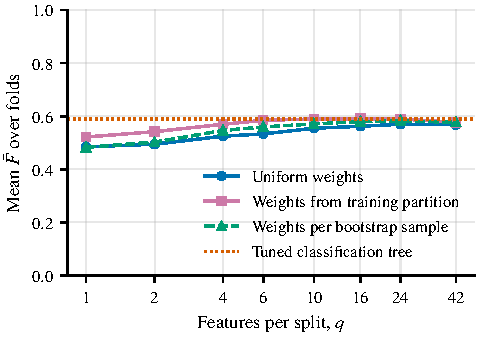
\includegraphics[width=0.49\textwidth]{rf_q_a.pdf}\label{fig:q-a}}\hfill
\subfloat[Strength and agreement under class weights]{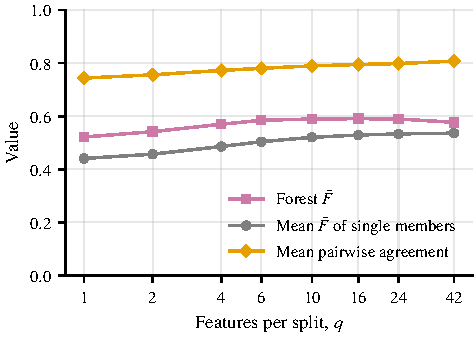
\includegraphics[width=0.49\textwidth]{rf_q_b.pdf}\label{fig:q-b}}
\caption{Effect of the number of features sampled per split}
\label{fig:q}
\end{figure*}

Figure~\ref{fig:q-a} shows that $\bar{F}$ rose steeply from one to six
features per split and reached the optimum at 16 or 24 features under every
weighting scheme. The best configuration used 16 features, with
weights computed once from the training partition, at $\bar{F} = 0.591$.
The bagged equivalent, with all 42 features, attained 0.577, so random
feature selection added 0.014 to plain bagging at equal weighting. The
recommended default of $\sqrt{p}$, equivalent to six features, attained
0.585 and was therefore suboptimal for the dataset. The result
supports the recommendation by Probst \textit{et al.}~\cite{probst2019} that
$q$ be tuned rather than fixed.

Figure~\ref{fig:q-b} explains the location of the optimum through
Equation~(\ref{eq:bound}). The mean $\bar{F}$ of a single member, a proxy
for the strength $s$, increased monotonically with $q$, from 0.441 at one
feature to 0.536 at 42 features. The mean pairwise agreement, a proxy for
the correlation $\bar{\rho}$, also increased monotonically, from 0.743 to
0.807. The gain of the forest over the mean member shrank as the agreement
grew: 0.081 at one feature, 0.062 at 16 features, and 0.041 at 42 features.
Small subsets therefore produced diverse but weak members, large subsets
produced strong but redundant members, and the optimum lay where the
increase in strength no longer compensated for the loss of diversity. The
agreement remained above 0.74 even at one feature per split, which is high
for an ensemble of fully grown trees. Part of the agreement arose from records that every member necessarily
misclassifies in the same way.

Class weighting remained beneficial inside the ensemble, which answers the
fifth research question. At 16 features per split, weights computed from the
training partition raised $\bar{F}$ from 0.562 to 0.591, a gain of 0.029,
against a gain of 0.018 for the single tree under the entropy criterion.
Averaging does not correct the bias of every member toward the majority
categories, because the members share the same bias, so the correction must
be applied to every member. Weights recomputed for every bootstrap sample
performed worse than weights computed once, by 0.011 at 16 features. The
experiments did not isolate the cause of the difference.

\subsection{Tree complexity within the forest}
\label{sec:res-complexity}

Figure~\ref{fig:complexity} presents the results of the second stage, which
addressed the fourth research question.

\begin{figure*}[!t]
\centering
\subfloat[Minimum leaf size]{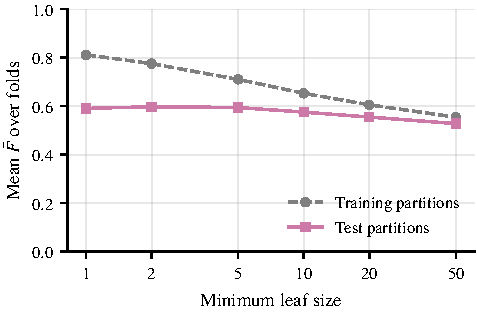
\includegraphics[width=0.49\textwidth]{rf_leaf.pdf}\label{fig:leaf}}\hfill
\subfloat[Maximum depth]{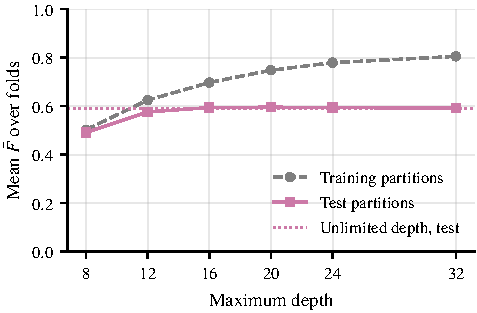
\includegraphics[width=0.49\textwidth]{rf_depth.pdf}\label{fig:depth}}
\caption{Effect of tree complexity limits on the random forest}
\label{fig:complexity}
\end{figure*}

The forest was far less sensitive to the depth limit than the single tree.
A depth limit of 16 raised the $\bar{F}$ of the single tree by 0.028 over
the unlimited tree, but raised the $\bar{F}$ of the forest by only 0.004,
from 0.591 to 0.594. Figure~\ref{fig:depth} shows that the training $\bar{F}$
of the forest grew steadily with depth while the test $\bar{F}$ remained
flat above a depth of 16. The average absorbed the additional variance of the deeper
members, as predicted in Section~\ref{sec:bg-ensemble}. A depth limit of eight or 12 reduced
performance sharply, because shallow members lack the capacity to isolate
the small categories, and averaging does not remove bias.

Figure~\ref{fig:leaf} shows that a minimum leaf size of two produced the
best forest overall, at $\bar{F} = 0.598$, while larger leaves reduced
performance steadily. A leaf of two instances prevents a member from fitting
a single conflicting record, and the effect is consistent with the report by
Probst \textit{et al.}~\cite{probst2019} that a small leaf size limit helps on
noisy data. The answer to the fourth research question is therefore that
the limits required by the single tree are largely unnecessary inside the
forest, and that only the mildest limit helped.

The training $\bar{F}$ of the fully grown forest was only 0.812, far below
the value of one that a perfect fit of the training data would produce. The
shortfall reflects the label conflicts of Section~\ref{sec:dataset}: a
group of identical feature vectors receives a single prediction, so every
record of the group with a different category is a training error that no
depth removes.

\subsection{Number of trees}
\label{sec:res-trees}

Figure~\ref{fig:trees} presents $\bar{F}$ as a function of $\tau$ for the
selected forest and for the bagged equivalent, which addresses the second
research question.

\begin{figure}[!t]
\centering
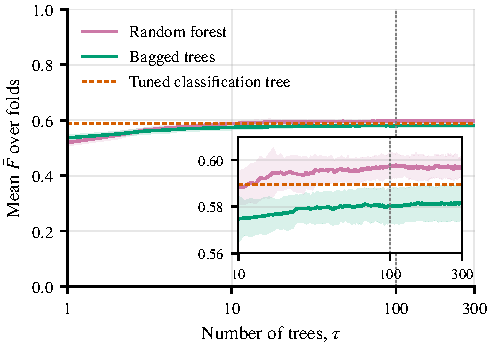
\includegraphics[width=\columnwidth]{rf_trees.pdf}
\caption{Performance as a function of the number of trees}
\label{fig:trees}
\end{figure}

The forest rose from $\bar{F} = 0.520$ with one tree to 0.588 with ten trees
and 0.596 with 50 trees, and then remained within 0.001 of 0.597 up to 300
trees. The selection rule of Section~\ref{sec:tune-rf} fixed $\tau$ at 100.
The highest value, 0.598, occurred at 110 trees, and the curve declined by
0.001 between 110 and 300 trees. The decline lay well within the fold-to-fold
standard deviation of 0.005, so the forest did not overfit as trees were
added, which agrees with the convergence result of
Breiman~\cite{breiman2001}. The small non-monotone variation matches the
observation of Probst and Boulesteix~\cite{probst2018} that measures other
than the error rate need not improve monotonically with $\tau$. Most of the
benefit of the ensemble was realised with 25 trees, which recovered
$96\,\%$ of the gain between one and 300 trees.

The bagged ensemble converged to $\bar{F} = 0.582$. The value equals the
cross-validated performance of the tuned tree on the same integer-coded
input, and lies below the value of 0.589 attained by the tree with indicator
encoding, which Figure~\ref{fig:trees} shows as the reference. Bootstrap
aggregation of trees with all 42 features therefore removed the need for a
depth limit, but did not improve on a well-tuned single tree. The entire advantage of the
forest arose from the random feature subsets.

\subsection{Performance on the generalisation set}
\label{sec:res-general}

Table~\ref{tab:final} reports the performance of the four tuned models on the
generalisation set, and Table~\ref{tab:tests} reports the paired statistical
comparisons.

\begin{table}[!t]
\centering
\caption{Performance on the generalisation set over ten seeds}
\label{tab:final}
\setlength{\tabcolsep}{3.5pt}
\begin{tabular}{@{}lcccc@{}}
\toprule
\textbf{Measure} & \textbf{Neighbours} & \textbf{Tree} & \textbf{Bagging} & \textbf{Forest} \\
\midrule
$\bar{F}$          & 0.459 & 0.591 & 0.589 & $\mathbf{0.607}$ \\
Deviation over seeds & 0 & 0.002 & 0.001 & 0.002 \\
$\bar{r}$          & 0.453 & $\mathbf{0.674}$ & 0.645 & 0.656 \\
$\eta$             & 0.769 & 0.752 & 0.781 & $\mathbf{0.785}$ \\
Training $\bar{F}$ & --    & 0.702 & 0.758 & 0.765 \\
Training (s)       & 0.5   & 4.0   & 55.6  & 23.7 \\
Prediction (s)     & 10.6  & 0.01  & 0.27  & 0.29 \\
\bottomrule
\end{tabular}
\end{table}

\begin{table}[!t]
\centering
\caption{Paired comparisons on the generalisation set, where $u$ and $v$ count the instances correct under the first and the second model only}
\label{tab:tests}
\setlength{\tabcolsep}{3pt}
\begin{tabular}{@{}lccrrc@{}}
\toprule
 & \multicolumn{2}{c}{\textbf{Bootstrap}} & \multicolumn{3}{c}{\textbf{McNemar test}} \\
\cmidrule(lr){2-3}\cmidrule(l){4-6}
\textbf{Comparison} & \textbf{Difference in} $\bar{F}$ & $p$ & $u$ & $v$ & $p$ \\
\midrule
Forest, tree       & $\phantom{-}0.016$ $[0.006, 0.027]$   & $<0.01$ & 2072 & 1007 & $<0.001$ \\
Forest, bagging    & $\phantom{-}0.019$ $[0.013, 0.026]$   & $<0.01$ & 705  & 557  & $<0.001$ \\
Forest, neighbours & $\phantom{-}0.148$ $[0.128, 0.165]$   & $<0.01$ & 2898 & 2381 & $<0.001$ \\
Tree, neighbours   & $\phantom{-}0.131$ $[0.111, 0.149]$   & $<0.01$ & 3017 & 3565 & $<0.001$ \\
Bagging, tree      & $-0.003$ $[-0.014, 0.008]$            & $0.57$  & 2027 & 1110 & $<0.001$ \\
\bottomrule
\end{tabular}
\end{table}

The forest attained the highest $\bar{F}$, at 0.607, against 0.591 for the
tree, 0.589 for bagging and 0.459 for the \gls{knn} model. The difference of
0.016 between the forest and the tree was significant after the Holm
adjustment, and the bootstrap interval of $[0.006, 0.027]$ excludes zero.
The answer to the first research question is therefore positive: the
\gls{rf} improved on the tuned tree, by a margin that is statistically
reliable but modest in size. The standard deviation over seeds was at most
0.002 for every tree-based model, so the ranking does not depend on the
seed. The performance of the tree and the \gls{knn} model on the
generalisation set lay within 0.01 of the cross-validated estimates of the
preceding study, which indicates that the leakage corrected in the present
study had only a small effect on the earlier estimates.

Bagging did not differ significantly from the tree in $\bar{F}$, yet the
bagged ensemble classified 2027 instances correctly that the tree missed,
against 1110 in the opposite direction, and raised $\eta$ from 0.752 to
0.781. The gains of bagging were therefore concentrated in the large
categories, where the gains add to $\eta$ but contribute little to an
unweighted mean over ten categories. The forest retained the accuracy gain
of bagging and added a gain in $\bar{F}$.

The three measures did not agree on a single winner. The forest led on
$\bar{F}$ and $\eta$, but the tree led on $\bar{r}$, at 0.674 against 0.656.
The \gls{knn} model was more accurate than the tree, with 3565 against 3017
instances classified correctly by one model only, yet trailed the tree by
0.131 in $\bar{F}$. Both disagreements arose from two specific categories.

\subsection{Performance per category}
\label{sec:res-perclass}

Figure~\ref{fig:perclass} presents $F_j$ per category for the four models,
and Figure~\ref{fig:confusion} presents the confusion matrix of the forest.

\begin{figure*}[!t]
\centering
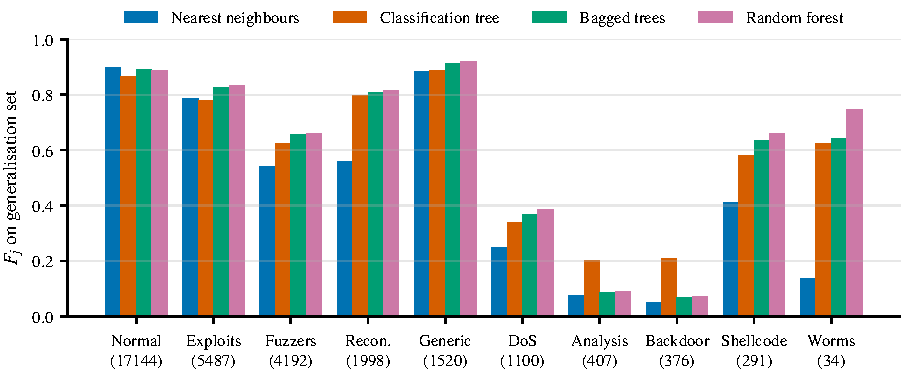
\includegraphics[width=\textwidth]{per_class.pdf}
\caption{Performance per category on the generalisation set, ordered by category size}
\label{fig:perclass}
\end{figure*}

\begin{figure}[!t]
\centering

\includegraphics[width=\columnwidth]{rf_confusion.pdf}
\caption{Row-normalised confusion matrix of the random forest, in percent}
\label{fig:confusion}
\end{figure}

Figure~\ref{fig:perclass} shows that the forest outperformed the tree on
eight of the ten categories, and outperformed bagging on nine. The gains
over the tree were largest on the small categories that remain separable:
0.122 on worms, 0.079 on shellcode and 0.049 on denial of service. The worms
estimate rests on only 34 test records and is the least reliable of the
ten. The forest performed worse than the tree on exactly two categories,
backdoor and analysis, where $F_j$ fell from 0.211 to 0.073 and from 0.203
to 0.091 respectively.

Figure~\ref{fig:confusion} shows the structure of the loss. The forest
assigned $58\,\%$ of the backdoor records to the analysis category, and
$50\,\%$ of the analysis records to the backdoor category, while recalling
only $16\,\%$ and $14\,\%$ of the two categories correctly. The two
categories were therefore not merely confused but systematically
exchanged. The tree, by contrast, recalled $44\,\%$ of the backdoor records
and $43\,\%$ of the analysis records, at a precision of only 0.14 and 0.13.
The high recall of the tree on the two categories explains the lead of the
tree on $\bar{r}$, which ignores precision. The same mechanism penalised the
\gls{knn} model, which recalled $6\,\%$ of the backdoor records and $5\,\%$
of the analysis records.

The remaining confusion of the forest lay in the block formed by the
denial of service, exploits, analysis and backdoor categories, and between
the fuzzers and normal categories, an overlap that Moustafa and
Slay~\cite{moustafa2016} reported in the original dataset.

\subsection{Effect of the label conflicts}
\label{sec:res-conflict}

The systematic exchange of the backdoor and analysis categories prompted an
analysis that was not planned before the evaluation. Deduplication retained
at most one record for every combination of feature values and category.
When a record of a conflicting group fell into the generalisation set, the
development partition therefore contained the same feature values under
other categories only. Of the \num{32549} generalisation records, 2294, or
$7.0\,\%$, had feature values that occur in the development partition, and
not one of the 2294 records had the own category among the development
records with identical features. The 2294 records include 304 of the 376
backdoor records and 314 of the 407 analysis records.

A model that reproduces the development label of an exact feature match must
misclassify every such record. The \gls{knn} model with distance weighting
assigns all weight to an exact match, and classified $1.0\,\%$ of the 2294
records correctly. The forest and bagging, with leaves of two instances,
classified $3.4\,\%$ and $3.2\,\%$ correctly. The depth-limited tree pools
neighbouring groups in large leaves, and classified $13.5\,\%$ correctly,
because the weighted majority of a pooled leaf occasionally matched the
held-out category. On the remaining \num{30255} records, $\bar{F}$ was 0.734
for the forest, 0.701 for bagging, 0.669 for the tree and 0.559 for the
\gls{knn} model. The advantage of the forest over the tree therefore grew
from 0.016 to 0.065 once the conflicting records were excluded.

The analysis has two consequences. First, the evaluation protocol penalises
low-bias models on conflicting records by construction, so the headline
comparison understates the advantage of the forest on records that the
features can separate. The lead of the tree on the backdoor and analysis
categories is an artefact of the interaction between deduplication and the
label conflicts, not evidence of a better model for the two categories.
Second, the conflicting records explain part of the high agreement between
forest members reported in Section~\ref{sec:res-q}, because every member
errs identically on such records. An empirical ceiling, computed as
described in Section~\ref{sec:ceiling-protocol}, yielded $\bar{F} = 0.808$
and $\eta = 0.944$, and limited $F_j$ to 0.35 for the backdoor category and
0.36 for the analysis category under the accuracy-optimal assignment. The
two categories are not separable from the 42 features, and no choice of
classifier changes that limit.

\subsection{Feature importance and computational cost}
\label{sec:res-cost}

Permutation importance on 8000 generalisation records ranked the
source-to-destination time to live first, with a reduction of 0.227 in
$\bar{F}$, followed by the source bytes at 0.203, the service at 0.154 and
the mean source packet size at 0.096. The impurity-based importance of the
same forest ranked the time to live only fourth. The time to live takes 13
distinct values, whereas the source bytes take 9382 distinct values, so the
difference between the two rankings reproduces the bias toward features
with many split points reported by Strobl
\textit{et al.}~\cite{strobl2007}, and supports the use of permutation
importance for the interpretation of the forest.

Table~\ref{tab:final} reports the computational cost of every model. The
forest trained in 23.7 seconds, about six times longer than the tree, and
classified the \num{32549} records in 0.29 seconds. Bagging trained in 55.6
seconds, because every split evaluated all 42 features rather than 16. The
forest was therefore both cheaper and better than bagging. The \gls{knn}
model required 36 times longer than the forest for prediction. An \gls{ids}
classifies traffic continuously and retrains infrequently, so the cost
profile of the forest suits the application.

%=====================================================================
\section{Conclusions}
\label{sec:conclusion}

The study evaluated a random forest (RF) for the classification of network
traffic records into ten categories, and compared the RF with a bagged
ensemble, a classification tree and a $k$-nearest neighbours (KNN) model on
a deduplicated version of the UNSW-NB15 dataset. All pre-processing was
fitted within the cross-validation folds, all tuning used a development
partition, and every model was evaluated once on a held-out generalisation
set.

The RF attained the highest macro-averaged $F_1$ measure on the
generalisation set, at 0.607 against 0.591 for the tuned tree, and the
difference was statistically significant. The improvement was modest. The
tuning of the RF answered the four remaining research questions. The
random feature subset was the source of the entire gain, because bagging
alone matched the tuned tree. The optimum of 16 features per split balanced
the strength of individual trees against the agreement between trees, and
the default of six features was suboptimal. Performance converged
at approximately 100 trees, and additional trees did not cause overfitting.
The depth limit that the single tree required became unnecessary inside the
ensemble, and only a minimum leaf size of two helped. Class weighting
remained necessary, because averaging does not correct a bias that every
member shares.

The most important finding concerned the data rather than the models. Of the
deduplicated records, $7.1\,\%$ share identical features with a record of a
different category, including approximately $80\,\%$ of the backdoor and
analysis records. Combined with deduplication, the conflicts guarantee the
misclassification of the affected held-out records by any model that
memorises exact matches. Excluding the affected records widened the
advantage of the RF over the tree from 0.016 to 0.065. The backdoor and
analysis categories are not separable from the available features.

Three directions for future work follow. The first direction is the
evaluation of the models on data with the original record multiplicities,
grouped by feature values so that identical records never span the training
and test partitions. The second direction is the merger of the backdoor and
analysis categories, or the acquisition of features that separate the two.
The third direction is a joint search over the control parameters of the
RF, which the computational budget of the study did not permit.
